\section{More Information More Balancing Strategies}
\label{sec:PADLB-proactstrategies}
\index{PADLB!Proactive Strategies}

We focus on the perspective of ``\textit{more information more balancing strategies}''. Almost all static load balancing solutions have to assume that they know about load, the number of tasks, or specific information about applications beforehand. After that, the problem can be formulated and solved by optimal algorithms. The optimal solutions also resolve the output: how many tasks are partitioned and which processes/MPI ranks are. We do not have this information ready at runtime for dynamic balancing problems. What we can have is usually queue length status and execution speed. The balancing strategies have to decide which tasks are migrated, from which rank to which rank. We know little about the execution speed based on the number of remaining tasks in queues per rank or even per machine. All in all, the outcome of almost balancing solutions resolves around:
\begin{enumerate}
	\item Which process shares tasks to which process?
	\item And, how many tasks should be migrated at a time?
\end{enumerate}

Differing from work stealing or reactive load balancing, we introduce a new scheme to perform load balancing more proactive. The approach enables task characterization and load prediction at runtime. We then use the prediction to provide the missing knowledge about load at runtime and guide task offloading. Therefore, as mentioned above, we have partial load information to calculate well (1) and (2). Additionally, we can generate different strategies for task offloading.\\

The context in this work is not static or a master-slave scheduling model\footnote{Where, tasks are generated automatically or nested during execution}. Our context is a given distribution of tasks in distributed memory machines. The approach is described as the runtime scheme shown in Figure \ref{fig:padlb_proact_scheme}. We leave one core off to run a dedicated thread along with other execution threads\footnote{Or so-called main threads to execute tasks of the parallel program.}. From the runtime point of view, we can see that our programs are performed with multiple processes or MPI ranks in distributed memory. In which each process spawns multiple threads to execute tasks, and each thread is pinned to one core. Notably, one dedicated thread is pinned to the last core to perform proactive load balancing. For modern computing architectures today, we have many sockets (even GPU as accelerators) in a single machine; a socket has many cores for parallel processing. At the operating system level, one process can spawn as many threads as recommended to fit the maximum number of physical cores per socket. Therefore, this scheme still fits reasonably to modern computing architectures today, even in the future.\\

%While the load balance is expected before running the applications, another challenge could be caused at the system side when some machines/processes can slow down. The unexpected situation needs actions at runtime and faces the challenge of moving tasks around to regain the balance as expected. Suppose there is no prior knowledge to redistribute the tasks. In that case, people have to use work-stealing ideas in principle, and the delay of stealing time on distributed memory is the challenge. Therefore, the approach in this thesis could be described in the inline figure below.\\

\begin{figure}[t]
	\centering
	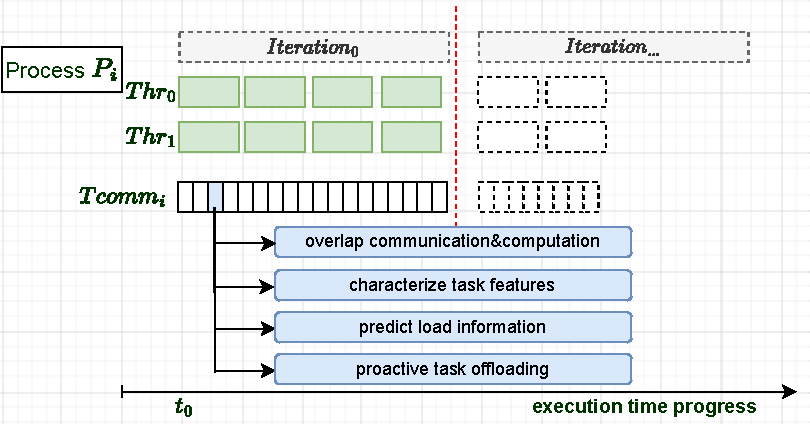
\includegraphics[scale=0.7]{./pictures/padlb_approach/padlb_proact_scheme.pdf}
	\caption{A proactive scheme for task offloading to solve dynamic load balancing in general.}
	\label{fig:padlb_proact_scheme}
\end{figure}

Figure \ref{fig:padlb_proact_scheme} shows our scheme at the level of one process running on one CPU socket. $T0$ and $T1$ illustrate the main execution threads for performing tasks. $Tcomm_{i}$ is the dedicated thread in this process. The x-axis shows the direction of execution time progress. Assume we have iterative execution such as $Iteration_{0}$ - the first execution phase, and so on ( $Iteration_{...}$). Compared to reactive load balancing, our approach extends $Tcomm_{i}$ to have the following properties as shown in Figure \ref{fig:padlb_proact_scheme}:

\begin{itemize}
	\item Because of leaving one core off anyway, $Tcomm$ run asynchronously and plays a role as an assistant for overlapping communication and computation.
	\item $Tcomm$ performs load monitoring, task characterizing, or even system information profiling.
	\item Generating load prediction model on-the-fly.
	\item Provide proactive task offloading to balance the load when necessary.
\end{itemize}

\begin{figure}[t]
  \centering
  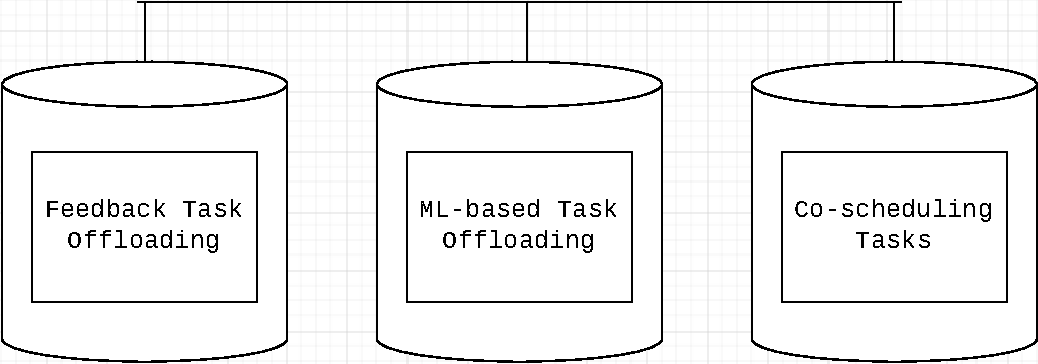
\includegraphics[scale=0.625]{./pictures/padlb_approach/padlb_three_branches_proact_strategies.pdf}
	\caption{Three branches of task offloading strategies for proactive load balancing approach.}
	\label{fig:three_branches_proact_strategies}
\end{figure}

The above properties are what $Tcomm$ can be enabled to do at runtime because it is managed separately from the other threads. Furthermore, we can define it adaptively in application-specific or system-specific domains. This scheme motivates us the idea of one approach toward different task offloading strategies to balance the load. Concretely, we can combine or adjust these properties to make different strategies. We show three strategies in this work as Figure \ref{fig:three_branches_proact_strategies} shows.\\

The first branch is feedback task offloading. The idea behind it is considered as an improved variant of reactive approaches. In terms of iterative applications, the first iteration is still applied reactive balancing operations. Tasks are offloaded from a slow process to a fast one during execution. Unlike the original approach, after the first iteration, we use $Tcomm$ to generate a statistic about local tasks, offloaded tasks, and total load per rank. We can summarize the total load and offloading information over iterations based on the statistic. Following that, a priority function for task offloading is created to tune which process has higher priority for migrating tasks simultaneously. The main purpose is to collect feedback and improve the next iterations. Over time, we can adjust the balancing operations to be more proactive and better in the next iterations. \\

The second branch is ML-based task offloading for load balancing, where ``\textit{ML-based}'' is considered as an online load prediction module. The load value of each task or each process can be predicted on-the-fly, and we use this information to build an adaptive algorithm for balancing. The idea of this branch is to use runtime profiled data to learn runtime values. This is useful in providing knowledge for a balancing strategy. \\

The last branch is co-scheduling tasks for load balancing, where ``\textit{co-scheduling}'' means process-by-process can talk to each other. To be extended, we can think about co-scheduling tasks across multiple applications as an outlook. $Tcomm$ will be the contact person between two or more processes. After an iteration, it will share the information about the prediction, and each process can know the load status before a new iteration starts. Hence, each can plan to balance the load in advance.

%
%\paragraph{Formulation of Influence Parameters}
%\label{PADLB-formulation}
%
%Sed mi sem, commodo et enim a, molestie rutrum nisl. Aliquam sit amet bibendum dui. Nam finibus tempus augue at pretium. Curabitur condimentum magna leo, eu bibendum tellus congue id. Aliquam tempor sed lectus a venenatis. Ut ornare nunc sit amet urna maximus maximus. Nunc tincidunt ex at metus sagittis convallis sit amet ac mi. In luctus nunc sem, a facilisis justo luctus vel. Cras ultricies ex ut quam elementum, sed pharetra ligula tristique. Maecenas fringilla sodales magna quis iaculis. Pellentesque id libero imperdiet, vehicula libero in, fermentum est. Mauris imperdiet risus sit amet hendrerit vestibulum. Curabitur tincidunt enim dui, non auctor leo fringilla vitae. Donec in tellus vitae eros sollicitudin blandit a id neque. Curabitur ante nibh, cursus ut aliquet ultricies, ultricies eget velit. Proin massa ex, scelerisque at tincidunt ac, porta non nibh.
